% Indicate the main file. Must go at the beginning of the file.
% !TEX root = ../main.tex

%%%%%%%%%%%%%%%%%%%%%%%%%%%%%%%%%%%%%%%%%%%%%%%%%%%%%%%%%%%%%%%%%%%%%%%%%%%%%%%%
% 03_results
%%%%%%%%%%%%%%%%%%%%%%%%%%%%%%%%%%%%%%%%%%%%%%%%%%%%%%%%%%%%%%%%%%%%%%%%%%%%%%%%


\section{Results}
\label{results}

\subsection{Hyperparameter Tuning}%%%%%%%%%%%%%%%%%%%%%%%%%%%%%%%%%%%%%%%%%%%%%%

The detailed results of the Hyperparameter tuning are shown in table \ref{tab:hyperparameters_results}.
The ranking of the score according to the accuracy or the F1 score are similar but there are some differences.
As an example is the best performance according to the accuracy 0.706 with an F1 score of 0.571 while 
the best score according to the F1 score is 0.608 with an accuracy of 0.667 - so the best model
divers in the two scores.
It is quite difficult to find any obvious tendencies for the influence of the hyperparameters on the performance of the model.
Figure \ref{fig:hyperparameters_boxplot} shows the distribution of the accuracy comparing different different hyperparameters
grouped by the transformation used. There is a tendency visible for the MelSpectrogramm to work a bit better.
A smaller learning rate seems to deliver results a bit less distributed but the difference is not very big.
For the MelSpectrogram transformation the number of ResBlocks seems to have a bigger influence on the performance -
two seems not to be enough. Furthermore there is a tendency for smaller kernel sizes to deliver less distributed results
but a better performance is achieved with a kernel size of 5. In figure \ref{fig:hyperparameters_scatterplot} the
models size measured by the number of trainable parameters is plotted against the accuracy and the F1 score.
There is no obvious correlation visible between the model size and the performance of the model.
This is also supported by the results of the Pearson Test. For both metrics the p value is far above 0.05 leaving the null hypothesis
that there is no significant correlation between the model size and the performance of the model.
The r values both quite close to zero but negative indicate that there might be a slight tendency for a smaller model to perform better.
The F1 score per class is shown in figure \ref{fig:f1_per_class} and compared to the distribution
of the available data. Class 11 has a very low F1 score compared to the available data while class 9 has a very high F1 Score
compared to the available data. To further examine the relation between the F1 score and the distribution of the data
in figure \ref{fig:f1_per_class_to_data_distribution} the F1 score is plotted against the distribution of the training data.
There is no obvious correlation visible between the F1 score and the distribution of the data. This is also supported by the results
of the Pearson Test. The p value is above 0.05 leaving the null hypothesis that there is no significant correlation. The r value
is positive therefore there might be a slight tendency for more training data to deliver a better F1 score.

%==== figure: hyperparameters_boxplot ====%
\begin{figure}[h]
\centering
\captionsetup{width=0.9\linewidth}
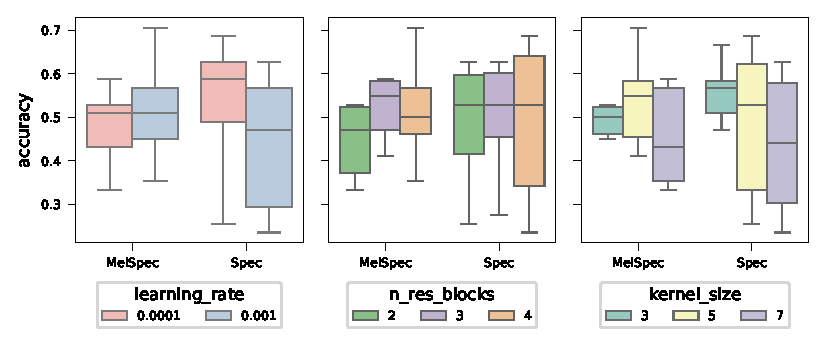
\includegraphics[width=1.0\textwidth]{figures/hyperparameters_boxplot.pdf}
\caption{Accuracy of the models for different hyperparameter grouped by the transformation type.}
\label{fig:hyperparameters_boxplot}
\end{figure}

%=========================================%

%==== figure: hyperparameters_scatterplot ====%
\begin{figure}[h]
\centering
\captionsetup{width=0.9\linewidth}
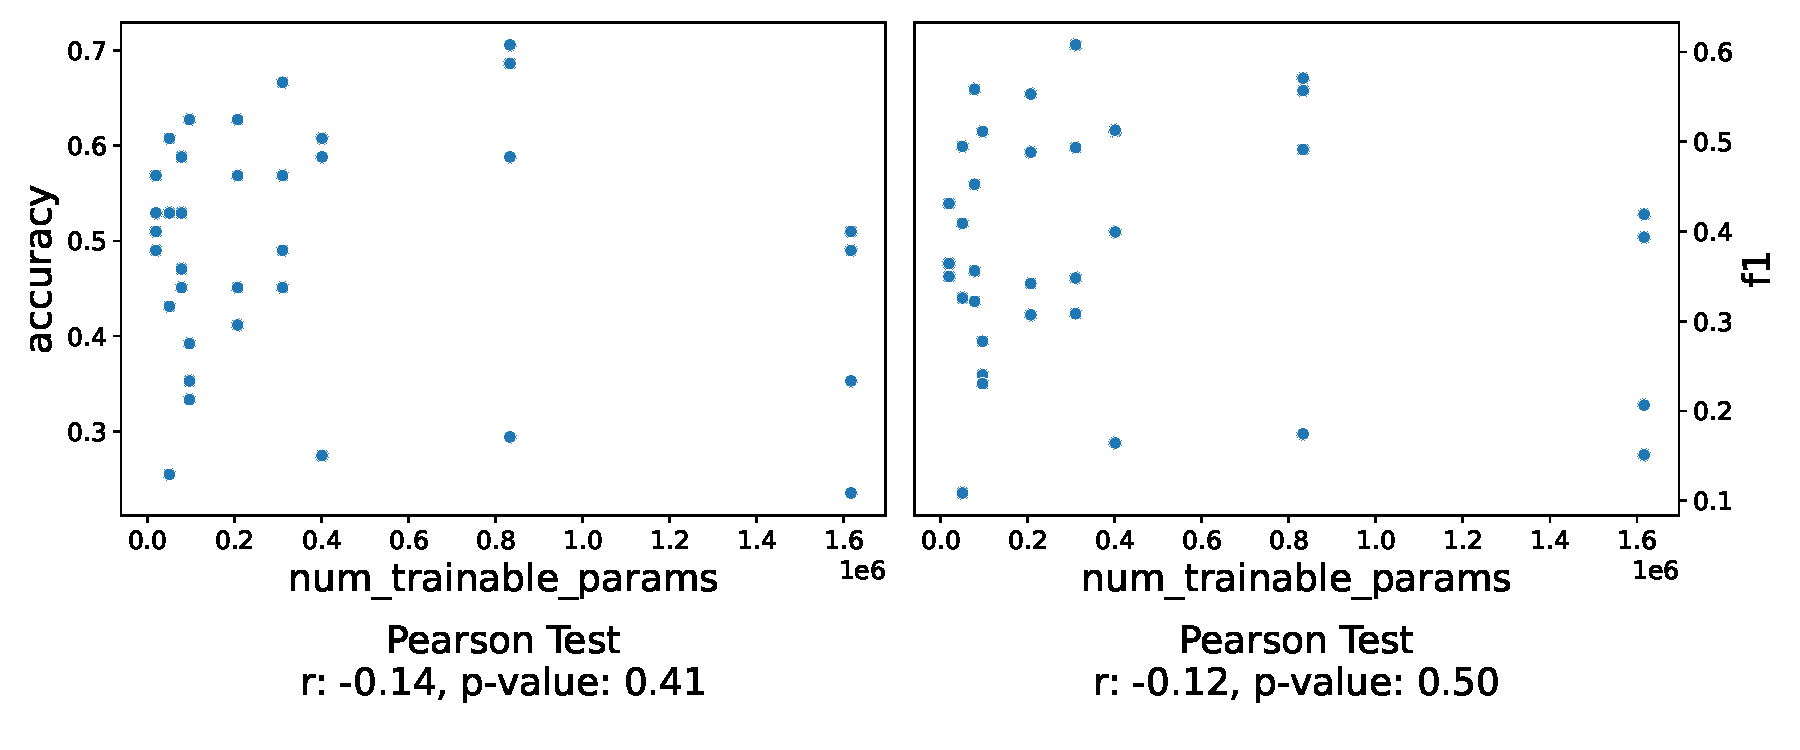
\includegraphics[width=1.0\textwidth]{figures/hyperparameters_scatterplot.pdf}
\caption{Model size compared to the accuracy and F1 Score of the models.}
\label{tab:hyperparameters_scatterplot}
\end{figure}

%=============================================%

%==== figure: f1_per_class ====%
\begin{figure}[h]
\centering
\captionsetup{width=0.9\linewidth}
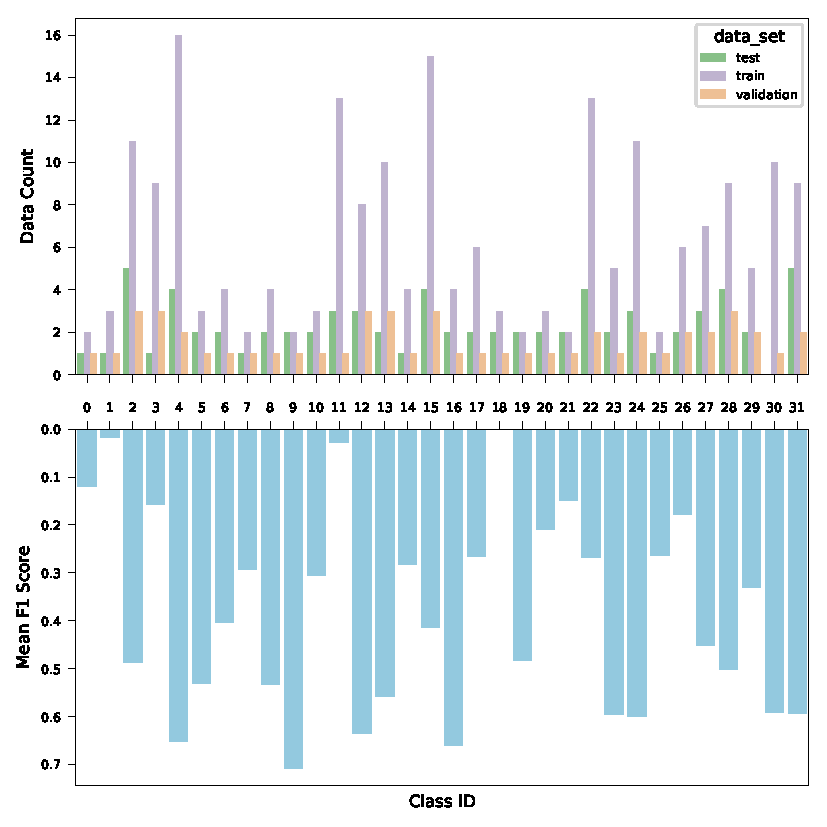
\includegraphics[width=1.0\textwidth]{figures/f1_per_class.pdf}
\caption{F1 Score per class as mean trough all models compared to data distribution.}
\label{tab:f1_per_class}
\end{figure}

%==============================%

%==== figure: f1_per_class_to_data_distribution ====%
\begin{figure}[h]
\centering
\captionsetup{width=0.8\linewidth}
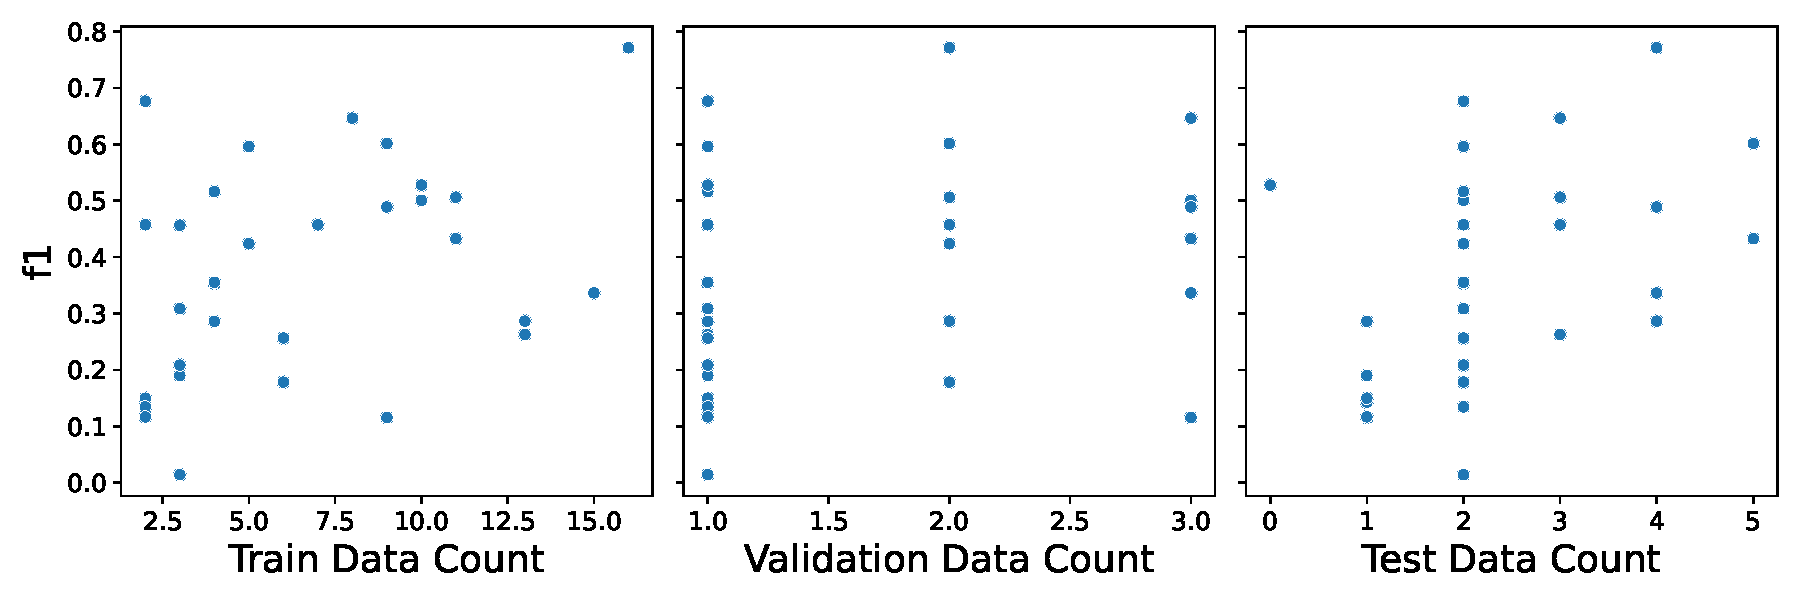
\includegraphics{figures/f1_per_class_to_data_distribution.pdf}
\caption{Available training data per classes compared to the F1 Score per classes in a scatter plot and the result of the Pearson correlation test.}
\label{fig:f1_per_class_to_data_distribution}
\end{figure}

%===================================================%


\subsection{Performance of the best Model}%%%%%%%%%%%%%%%%%%%%%%%%%%%%%%%%%%%%%%

The best performing configuration for the model was found to be the one with the following hyperparameters:

\begin{itemize}
    \item \textbf{n\_mels:} 64
    \item \textbf{n\_res\_blocks:} 4
    \item \textbf{learning\_rate:} 0.001
    \item \textbf{kernel\_size:} 5
\end{itemize}

On the test set, the model achieved an accuracy of 0.649 and an F1 score of 0.546. 
The confusion matrix for the predictions generated by this model is shown in Figure \ref{fig:confusion_matrix_best}.
The concentration of results in the diagonal of the confusion matrix indicates that the model is performing well.
Class 22 was predicted the most frequent with more than 50\% of the predictions being wrong.

%==== figure: confusion_matrix_best ====%
\begin{figure}[h]
\centering
\captionsetup{width=0.9\linewidth}
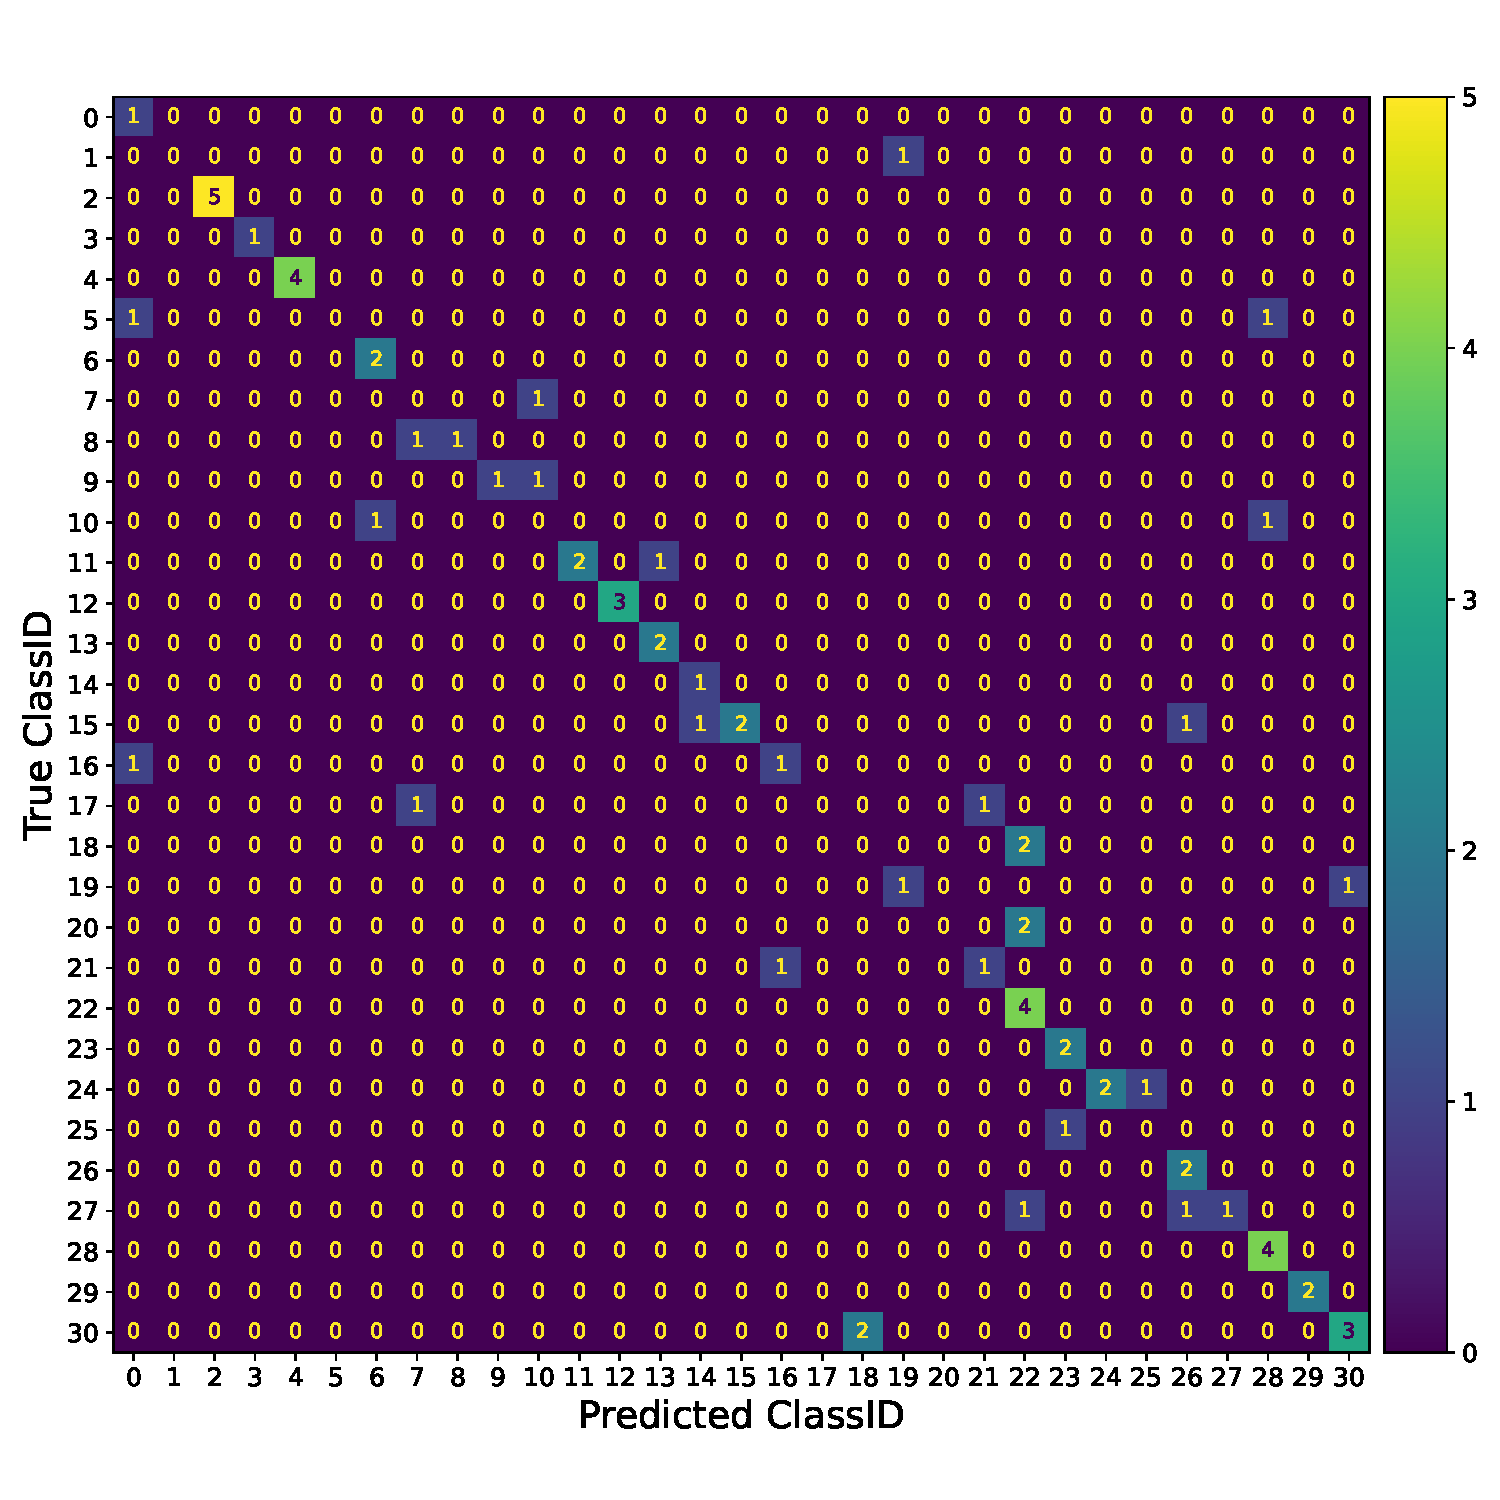
\includegraphics[width=1.0\textwidth]{figures/confusion_matrix_best.pdf}
\caption{Confusion matrix for the predictions of the test set using the best model. The over all accuracy on the test set was 0.649.}
\label{tab:confusion_matrix_best}
\end{figure}

%=======================================%
